\documentclass{tufte-handout}

% ams
\usepackage{amssymb,amsmath}

% utf8 encoding
\usepackage[utf8]{inputenc}

% graphix
\usepackage{graphicx}
\setkeys{Gin}{width=\linewidth,totalheight=\textheight,keepaspectratio}

% booktabs
\usepackage{booktabs}

% url
\usepackage{url}

% hyperref
\usepackage{hyperref}

% units.
\usepackage{units}

% pandoc syntax highlighting
\usepackage{color}
\usepackage{fancyvrb}
\newcommand{\VerbBar}{|}
\newcommand{\VERB}{\Verb[commandchars=\\\{\}]}
\DefineVerbatimEnvironment{Highlighting}{Verbatim}{commandchars=\\\{\}}
% Add ',fontsize=\small' for more characters per line
\newenvironment{Shaded}{}{}
\newcommand{\KeywordTok}[1]{\textcolor[rgb]{0.00,0.44,0.13}{\textbf{{#1}}}}
\newcommand{\DataTypeTok}[1]{\textcolor[rgb]{0.56,0.13,0.00}{{#1}}}
\newcommand{\DecValTok}[1]{\textcolor[rgb]{0.25,0.63,0.44}{{#1}}}
\newcommand{\BaseNTok}[1]{\textcolor[rgb]{0.25,0.63,0.44}{{#1}}}
\newcommand{\FloatTok}[1]{\textcolor[rgb]{0.25,0.63,0.44}{{#1}}}
\newcommand{\CharTok}[1]{\textcolor[rgb]{0.25,0.44,0.63}{{#1}}}
\newcommand{\StringTok}[1]{\textcolor[rgb]{0.25,0.44,0.63}{{#1}}}
\newcommand{\CommentTok}[1]{\textcolor[rgb]{0.38,0.63,0.69}{\textit{{#1}}}}
\newcommand{\OtherTok}[1]{\textcolor[rgb]{0.00,0.44,0.13}{{#1}}}
\newcommand{\AlertTok}[1]{\textcolor[rgb]{1.00,0.00,0.00}{\textbf{{#1}}}}
\newcommand{\FunctionTok}[1]{\textcolor[rgb]{0.02,0.16,0.49}{{#1}}}
\newcommand{\RegionMarkerTok}[1]{{#1}}
\newcommand{\ErrorTok}[1]{\textcolor[rgb]{1.00,0.00,0.00}{\textbf{{#1}}}}
\newcommand{\NormalTok}[1]{{#1}}

% multiplecol
\usepackage{multicol}

% lipsum
\usepackage{lipsum}

% title / author / date
\title{Introducción a la Representación del Conocimiento \textbar{} MRC}
\author{Víctor Peinado
\href{mailto:v.peinado@filol.ucm.es}{v.peinado@filol.ucm.es}}
\date{3-9 de octubre de 2014}


\begin{document}

\maketitle



\section{Referencias}\label{referencias}

\begin{itemize}
\itemsep1pt\parskip0pt\parsep0pt
\item
  (Brachman \& Levesque, 2004, chap. 1) \footnote{Brachman, R.;
    Levesque, H. \emph{Knowledge Representation and Reasoning}. Morgan
    Kaufmann. 2004.
    \url{http://rair.cogsci.rpi.edu/pai/library/brachmanbook7-17-03.pdf}}
\item
  Presentación con los contenidos del libro, por H. Levesque \footnote{\url{http://www.cs.toronto.edu/~hector/PublicKRSlides.pdf}}
\item
  (van Harmelen, Lifschitz, Porter, 2008, chap. 1) \footnote{van
    Harmelen, Lifschitz, V. Porter, B. (Eds.) \emph{Handbook of
    Knowledge Representation}. Elsevier Science. 2008.
    \url{http://dai.fmph.uniba.sk/~sefranek/kri/handbook/}}
\item
  Videolectures: \emph{Knowledge Representation and Reasoning}
  \footnote{Videolectures: \emph{Knowledge Representation and
    Reasoning}. \url{http://videolectures.net/ssll09_pagnucco_krr/}}
\end{itemize}

\section{Algo de contexto}\label{algo-de-contexto}

La \textbf{inteligencia}, o al menos, el comportamiento inteligente, es
una de las características clave que nos definen como seres humanos y
que parecen situar una línea divisoria entre nosotros por un lado, y los
grandes simios, algunos mamíferos\ldots{} y el resto del reino animal.

En los humanos, este \textbf{comportamiento inteligente} viene
determinado por el \emph{conocimiento} que manejamos: cuando actuamos
tomando decisiones, lo hacemos basándonos en lo que sabemos acerca del
mundo. Cuando actuamos racionalmente, lo hacemos en base a lo que
sabemos o creemos
saber.\marginnote{Es más, cuando no actuamos racionalmente o tomamos decisiones claramente equivocadas, lo justificamos diciendo que hemos actuado sin pensar.}

La \textbf{Inteligencia Artificial} (IA) es la
disciplina\marginnote{La IA es una área multidisciplinar (computación, ingeniería, psicología, filosofía...) que aparentemente solo se estudia en Escuelas de Informática}
encargada del estudio del comportamiento inteligente alcanzado a través
de medios computacionales. Dentro de esta Inteligencia Artificial,
podemos identificar la \emph{representación del conocimiento y el
razonamiento} como el área relacionada con el estudio de \emph{actores}
que utilizan el conocimiento que poseen para decidir qué hacer y cómo
actuar: es el estudio del pensamiento como proceso computacional llevado
a cabo por máquinas.

\section{¿Qué es el conocimiento?
\marginnote{Definir qué es el conocimiento parece una tarea más propia de filósofos y objeto de conversaciones metafísicas. Somos modestos y nos basta con dar una definición informal.}}\label{que-es-el-conocimiento}

Cuando decimos cosas como ``Pepito sabe que\ldots{}'' podemos rellenar
el hueco con cualquier oración declarativa. P. ej., ``Pepito sabe que
Manolita viene a la fiesta'', o ``Pepito sabe que el Atleti ganó el
último partido''.

En este sentido, el conocimiento parece ser una relación entre alguien
que sabe algo (Pepito) y una \emph{proposición}, una idea expresada a
través de una oración declarativa.

Una \textbf{proposición} no es más que una entidad abstracta que pueden
ser verdadera o falsa, que puede ser acertada o incorrecta. Cuando
decimos cosas como ``Pepito sabe que \emph{p}'', en realidad queremos
decir que Pepito sabe (o cree) que \emph{p} es
verdad.\marginnote{¿Es equivalente saber y creer que se sabe algo?}
Decir que Pepito sabe algo implica que Pepito se ha formado un juicio de
algún tipo que le ha llevado a pensar que el mundo es de determinada
forma, y no de otra.

Existe por lo tanto un tipo de oraciones que utilizan verbos como
\emph{saber, esperar, arrepentirse, temer,
dudar}\marginnote{Ojo, hay oraciones que contienen estos verbos que no incluyen de manera explícita proposiciones. P. ej., "Juanito sabe cómo llegar", "María sabe tocar la guitarra", "Pepito teme a los perros" no contienen proposiciones.}
que parecen denotar relaciones entre actores y proposiciones. En estos
casos, lo realmente importante acerca de las proposiciones es un valor
de verdad. ``Pepito espera que Manolita venga a la fiesta'' implica que
Pepito espera que el mundo sea de una forma de terminada, y no de otra.

Una idea relacionada es la de \textbf{creencia}. ``Pepito cree que
\emph{p}'' está directamente relacionada con ``Pepito sabe que
\emph{p}''. Si acaso, utilizamos la primera cuando no queremos afirmar
tajantemente que el juicio de Pepito es exacto o cuando no está
convencido. Existen ejemplos de oraciones que expresan distintos grados
de actitudes proposicionales: ``Pepito está totalmente seguro de que
\emph{p}'', ``Pepito está convencido de que \emph{p}'', ``Pepito es de
la opinión de que \emph{p}'', ``Pepito sospecha que \emph{p}''. En todas
ellas, en distinto grado, Pepito asume que el mundo es de una
determinada forma, y no de otra.

\section{¿Qué es representación?}\label{que-es-representacion}

\textbf{Representación} es la relación que se establece entre dos
dominios o ámbitos (un representante y una cosa representada) de manera
que el primero \emph{significa} o \emph{toma el lugar} de la segunda.
\marginnote{Pictogramas: peligro de cocodrilos, prohibido el baño}

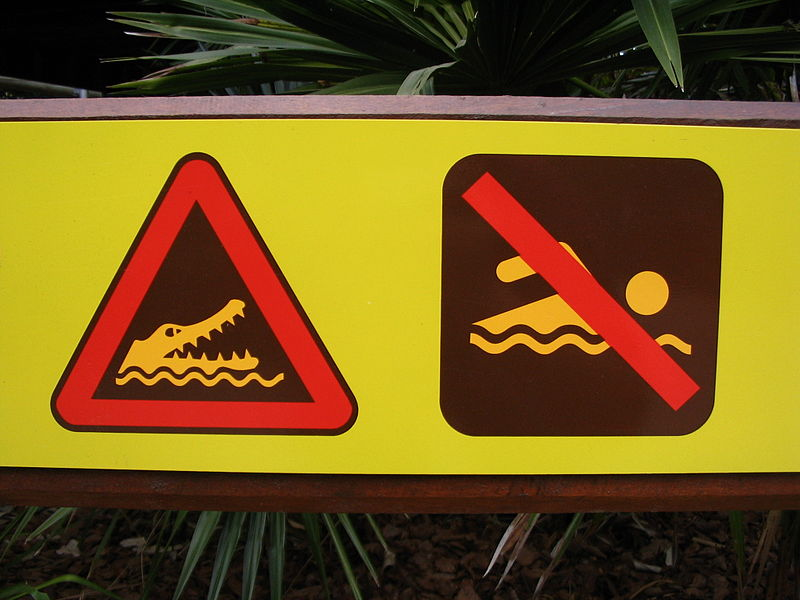
\includegraphics{img/pictogram.jpg}

El tipo de representante que más nos interesa en esta asignatura es el
\textbf{símbolo}. El símbolo \emph{7} significa \emph{número 7}, y es
equivalente en otros contextos a los símbolos \emph{siete},
\emph{seven}, \emph{VII}, \emph{qi}. Estos símbolos son, habitualmente,
más accesibles y fáciles de manejar que los objetos que representan. Por
eso los manipulamos y realizamos operaciones de cálculo con ellos.

Es\marginnote{La representación simbólica es concreta, contiene elementos que podemos segmentar y manejar por separado. Sin embargo, la proposición es una entidad abstracta que nos permite distinguir dos tipos de mundos imaginables: aquellos en los que es verdad que Pepito ama a Manolita, y aquellos en los que este amor es imposible.}
importante distinguir claramente cuando una secuencia o conjunto de
símbolos formales representan una proposición: ``Pepito ama a Manolita''
es el conjunto de símbolos que significa que Pepito ama a Manolita.

Por lo tanto, la \textbf{representación del conocimiento} es el campo de
estudio relacionado con la utilización de símbolos formales para
representar una colección de proposiciones que algún actor conoce o cree
conocer. Aunque un determinado actor conozca o crea conocer un número
muy grande de proposiciones, es imposible representarlas explícitamente
todas. De hecho, va a existir siempre una brecha entre el conocimiento
representado y el que realmente manejamos. Aquí es donde entra el
\emph{razonamiento}.

\section{¿Qué es razonamiento?}\label{que-es-razonamiento}

Por \textbf{razonamiento} entendemos la manipulación formal de los
símbolos que representan las proposiciones conocidas por un actor para
producir representaciones de proposiciones nuevas. Es precisamente aquí
donde aprovechamos la naturaleza concreta y accesible de los
representantes: los localizamos, manipulamos, modificamos y creamos
nuevas representaciones.

Como analogía del
razonamiento,\marginnote{Este ejemplo de razonamiento recibe el nombre de \textit{inferencia lógica}. De acuerdo con esta visión, el razonamiento es una forma de cálculo, no muy diferente de la aritmética, en la que manipulamos símbolos que representan proposiciones en lugar de números.}
pensemos en las operaciones aritméticas. A partir de dos símbolos,
podemos realizar sumas, restas, divisiones\ldots{} para generar nuevos
símbolos. El razonamiento funciona de manera similar. A partir de
símbolos como ``Todos los hombres son mortales'', ``Pepito es un
hombre'', tras realizar determinadas operaciones de manipulación,
podemos producir el símbolo ``Pepito es mortal''.

\section{¿Por qué el conocimiento es importante para la
IA?}\label{por-que-el-conocimiento-es-importante-para-la-ia}

A menudo es útil describir el comportamiento de sistemas complejos
utilizando metáforas como objetivos, intenciones, creencias, esperanzas.
Es habitual describir un sistema de IA en términos intencionales porque
es sencillo explicar el comportamiento a partir de los objetivos y
creencias que
maneja.\marginnote{El ejemplo típico es el del sistema capaz de jugar al ajedrez: el ordenador \textit{sabe} dónde están las piezas y \textit{quiere} ganar la partida accoralando al rey....}

Esta descripción basada en supuestas intenciones y objetivos se conoce
como \emph{actitud/postura intencional}. Y aunque este tipo de
antopomorfización no siempre es adecuada a la hora de describir el
funcionamiento de cualquier sistema, en IA se utiliza para justificar la
construcción de \textbf{sistemas basado en el conocimiento}
(\emph{knowledge-based systems}) que manejan conjuntos de
representaciones simbólicas llamadas \textbf{bases de conocimiento}
(\emph{knowledge bases}).

\section{Sistemas basados en
conocimiento}\label{sistemas-basados-en-conocimiento}

Los siguientes dos programas en Prolog producen el mismo resultado:
imprimen por pantalla el color de distintos objetos. Es más, podemos
describir sus comportamientos como intencionales.

Alternativa 1:

\begin{Shaded}
\begin{Highlighting}[]
\NormalTok{imprimeColor(nieve) }\KeywordTok{:-} \KeywordTok{!,} \FunctionTok{write}\NormalTok{(}\OtherTok{"}\ErrorTok{Es}\AlertTok{ }\ErrorTok{blanco}\OtherTok{."}\NormalTok{)}\KeywordTok{.}
\NormalTok{imprimeColor(hierba) }\KeywordTok{:-} \KeywordTok{!,} \FunctionTok{write}\NormalTok{(}\OtherTok{"}\ErrorTok{Es}\AlertTok{ }\ErrorTok{verde}\OtherTok{."}\NormalTok{)}\KeywordTok{.}
\NormalTok{imprimeColor(cielo) }\KeywordTok{:-} \KeywordTok{!,} \FunctionTok{write}\NormalTok{(}\OtherTok{"}\ErrorTok{Es}\AlertTok{ }\ErrorTok{amarillo}\OtherTok{."}\NormalTok{)}\KeywordTok{.}
\NormalTok{imprimeColor(}\DataTypeTok{Cosa}\NormalTok{) }\KeywordTok{:-} \FunctionTok{write}\NormalTok{(}\OtherTok{"}\ErrorTok{No}\AlertTok{ }\ErrorTok{lo}\AlertTok{ }\ErrorTok{sé}\AlertTok{ }\OtherTok{:-/"}\NormalTok{)}\KeywordTok{.}
\end{Highlighting}
\end{Shaded}

Alternativa 2:

\begin{Shaded}
\begin{Highlighting}[]
\NormalTok{imprimeColor(}\DataTypeTok{Cosa}\NormalTok{) }\KeywordTok{:-} \NormalTok{color(}\DataTypeTok{Cosa}\KeywordTok{,} \DataTypeTok{Color}\NormalTok{)}\KeywordTok{,} \KeywordTok{!,} \FunctionTok{write}\NormalTok{(}\OtherTok{"}\ErrorTok{Es}\AlertTok{ }\OtherTok{"}\NormalTok{)}\KeywordTok{,} \FunctionTok{write}\NormalTok{(}\DataTypeTok{Color}\NormalTok{)}\KeywordTok{,} \FunctionTok{write}\NormalTok{(}\OtherTok{"."}\NormalTok{)}\KeywordTok{.}
\NormalTok{imprimeColor(}\DataTypeTok{Cosa}\NormalTok{) }\KeywordTok{:-} \FunctionTok{write}\NormalTok{(}\OtherTok{"}\ErrorTok{No}\AlertTok{ }\ErrorTok{lo}\AlertTok{ }\ErrorTok{sé}\AlertTok{ }\OtherTok{:-/"}\NormalTok{)}\KeywordTok{.}

\NormalTok{color(nieve}\KeywordTok{,} \NormalTok{blanco)}\KeywordTok{.}
\NormalTok{color(cielo}\KeywordTok{,} \NormalTok{amarillo)}\KeywordTok{.}
\NormalTok{color(}\DataTypeTok{Cosa}\KeywordTok{,} \DataTypeTok{Color}\NormalTok{) }\KeywordTok{:-} \NormalTok{estaHechoDe(}\DataTypeTok{Cosa}\KeywordTok{,} \DataTypeTok{Material}\NormalTok{)}\KeywordTok{,} \NormalTok{color(}\DataTypeTok{Material}\KeywordTok{,} \DataTypeTok{Color}\NormalTok{)}\KeywordTok{.}

\NormalTok{estaHechoDe(hierba}\KeywordTok{,} \NormalTok{vegetacion)}\KeywordTok{.}
\NormalTok{color(vegetacion}\KeywordTok{,} \NormalTok{verde)}\KeywordTok{.}
\end{Highlighting}
\end{Shaded}

Pero solo la alternativa 2 está basada en conocimiento porque tiene una
colección de representaciones simbólicas que representan proposiciones.
Entre otras cosas, contiene \emph{hechos} como
\texttt{color(nieve, blanco).} que representa de manera simbólica la
proposición ``el color de la nieve es blanco'', o como
\texttt{estaHechoDe(hierba, vegetacion).} que representa la proposición
``la hierba está hecha de vegetación''. Si elimináramos cualquiera de
estos hechos, el programa no contendría ese conocimiento y sería incapaz
de responder a la instrucción ``imprime el color de la nieve'' o
``imprime el color de la hierba''. En la alternativa 1 por el contrario,
no hay una colección de proposiciones, simplemente reglas del estilo
``si te preguntan por el color de la nieve, responde blanco''.

A simple vista, la alternativa 2 parece más compleja, ¿qué ventajas
tienen los sistemas basados en conocimiento? Son ideales para tareas
abiertas porque:

\begin{itemize}
\item
  permiten\marginnote{La hierba es verde porque está hecha de vegetación}
  justificar adecuadamente la toma de decisiones
\item
  son\marginnote{el cielo es azul, no amarillo} más fáciles de mantener
  y corregir cuando el comportamiento es erróneo
\item
  son\marginnote{Las rosas son rojas} sencillos de extender, añadiendo
  nuevo conocimiento
\item
  son\marginnote{Imprime por pantalla todos los objetos blancos que conozcas}
  sencillos de adaptar, añadiendo nuevas aplicaciones
\end{itemize}

\section{¿Por qué necesitamos
razonamiento?}\label{por-que-necesitamos-razonamiento}

Cuando construimos un sistema basado en conocimiento, queremos que actúe
teniendo en cuenta las creencias que tiene sobre el mundo, no solo sobre
el conocimiento que aparece representado de manera explícita en su base
de conocimiento. En la segunda alternativa del programa que hemos visto
antes, no aparece explícita ninguna representación simbólica que diga
``la hierba es verde'', y sin embargo el sistema es capaz de encontrar
que la hierba está compuesta de determinado material y sabe que este
material es verde, lo que conlleva que la hierba también es verde.

Cuando tenemos un conjunto \emph{S} de proposiciones representadas como
oraciones o hechos, y la verdad de una oración \emph{p} está implícita
en la verdad de \emph{S}, decimos que \emph{p} es \textbf{consecuencia
lógica} (\emph{entailment}) de \emph{S}, o que \emph{S} conlleva o
implica \emph{p}. Si el mundo es de tal manera que todos los elementos
de \emph{S} son verdaderos y \emph{S} implica \emph{p}, entonces
\emph{p} tiene que ser verdadero también.

La \textbf{inferencia} consiste en calcular consecuencias lógicas. Y
razonar consiste precisamente en calcular todas las consecuencias
lógicas de una base de conocimiento. Todo sistema que razone sobre una
base de conocimiento deberá proporcionar (¿todas?) las consecuencias
lógicas que pueda extraer del conocimiento explícito que maneja. Habrá
sistemas que no devuelva todas las respuestas posibles y otros que
devuelvan algunas incorrectas, pero en determinados contextos estos
sistemas serán preferibles a no tener respuestas.

\section{¿Por qué utilizamos Lógica?}\label{por-que-utilizamos-logica}

El uso de la lógica es relevante para representar conocimiento y llevar
a cabo razonamiento porque precisamente la lógica consiste en el estudio
de las consecuencias lógicas, y en el uso de lenguajes, condiciones de
verdad y reglas de inferencia. El primer lenguaje de representación del
conocimiento que vamos a utilizar está basado en la \textbf{lógica de
primer
orden}.\marginnote{Lógica de predicados, inventada por Frege para formalizar las matemáticas.}


\end{document}
